% SW design
\clearpage

\section{Software design}

Herunder er de forskellige dele af softwaren kort beskrevet. 

\subsection{PC delen (JC)}

Softwaren til PC'en, er brugeren grænseflade til at kontrollere systemet. Her kan han manurære rundt i de forskellige menuer og udføre de forskellige ting som er beskrevet i use casene.

Nedenfor er der illustreret hvordan man kommer frem og tilbage i brugerinterfacet. Udover bruger input så kan CSS hovedenheden give PC'en besked om at der ikke længere er logget ind hvilket vil sende brugeren fra main menu og tilbage til pre-login menuen. På grund af software begræsninger kan der kun sendes babyalarm så længe brugeren står i main menuen og ikke har trykket på keyboardet endnu.

\begin{figure}[htbp] \centering
{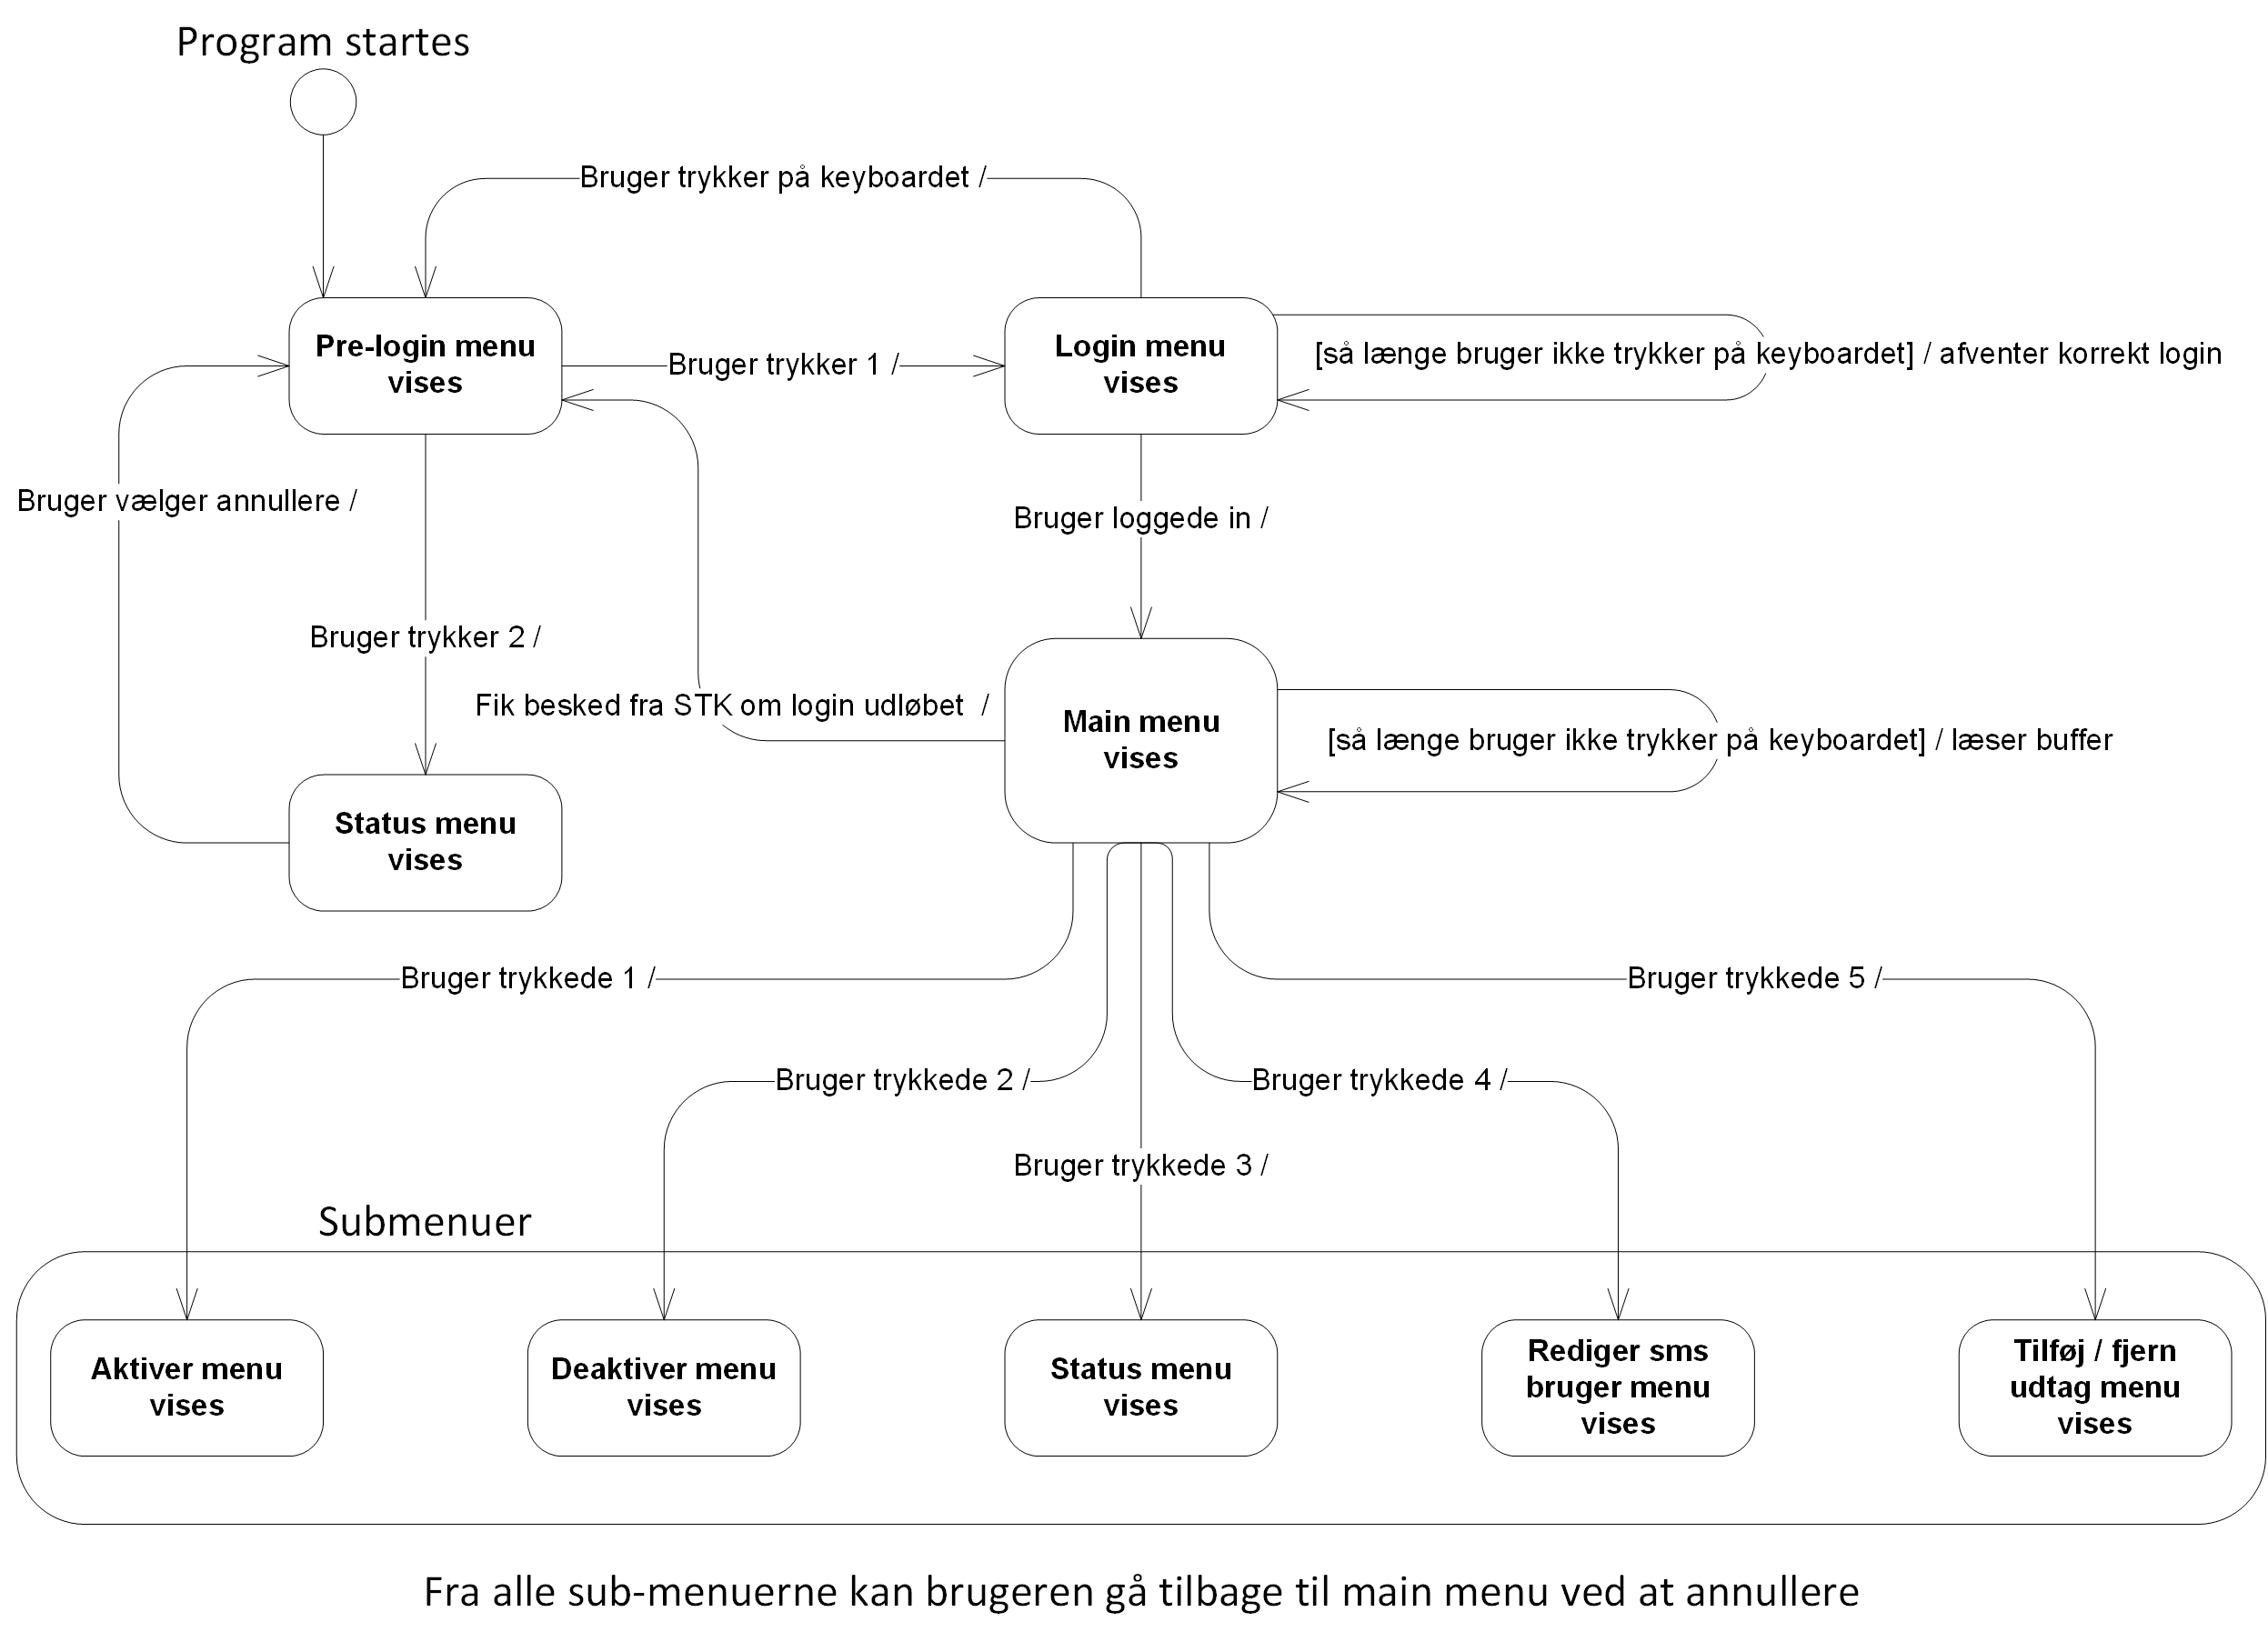
\includegraphics[width=\textwidth]{billeder/uml/state_machine_main}}
\caption{State machine diagram over brugerflade}
\label{fig:State machine diagram over brugerflade}
\end{figure}

En vigtig del af PC software er at vi kunne gemme alle de enheder brugeren har og hvilket telefonnummer brugeren har. Dette håndtere Hukommelse klassen som gemmer alt i en text fil og henter dataen ind under opstart. Således kan brugeren lukke programmet, åbne det igen og stadig have de samme enheder samt deres status og adresse. \ref{fig:Hukommelses header og udklip af text filen} Illustrere hvordan enhederne og telefonnummeret er gemt i text filen.

\begin{figure}[htbp] \centering
{\includegraphics[width=\textwidth]{billeder/uml/pc_dataview}}
\caption{Hukommelses header og udklip af text filen}
\label{fig:Hukommelses header og udklip af text filen}
\end{figure}